The Earth stands at a critical juncture in its history, where the consequences of human activity on the environment have reached a crossroads of global significance. Climate change, driven primarily by the relentless emission of greenhouse gases, has manifested itself in increasingly severe weather patterns, rising sea levels, and ecological disruptions. The urgency of the situation cannot be overstated, as nations grapple with the complex challenge of reducing carbon dioxide (CO$_2$) emissions to mitigate the impending climate crisis \cite{solomon2009irreversible,noaa-co2,world2016ambient}. 

The dire need for sustainable energy solutions has never been more evident. Various sectors of the economy are challenged to reduce their carbon footprint in order to restrict their impact on climate change. The transport sector was responsible for 23\% of global emissions from fuel combustion in 2021 and emerges as a critical contributor to the climate change predicament \cite{iea-transport}. 

\begin{figure}[h]
    \centering
    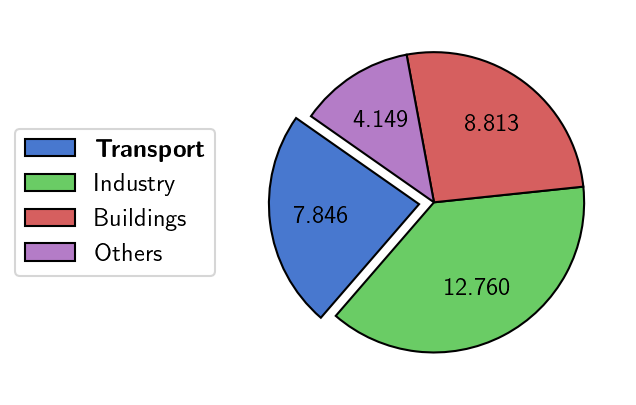
\includegraphics[width=0.75\textwidth]{Images/Chapter1/iea-transport.png}
    \caption{2021 Global CO$_2$ emissions from fuel combustion by sector [$\text{GtCO}_2$]. Source: IEA (2023) \cite{iea-transport}.}
    \label{fig:iea-transport}
\end{figure}

As societies evolve and the global population continues to grow, the demand for transportation, particularly in the form of automobiles and other fossil-fuel-reliant means, has risen dramatically. Innovative solutions are crucial to decouple the connection between personal mobility and CO$_2$ emissions. Electric vehicles (EVs) have emerged as a promising alternative to traditional internal combustion engine vehicles. They offer the potential to revolutionize the way we commute, significantly diminishing the transportation sector's contribution to carbon emissions. 

% \begin{figure}
%     \centering
%     
\includegraphics[width=0.7\textwidth]{Images/Chapter1/noaa-co2.png}
%     \caption{Trends in Atmospheric Carbon Dioxide. Source: NOAA (2023) \cite{noaa-co2}.}
%     \label{fig:noaa-co2}
% \end{figure}

At the heart of the electric vehicle industry's transformation lie lithium-ion batteries (LIBs). These energy storage devices have rapidly gained prominence as the primary means of powering EVs \cite{zubi2018lithium,stampatori2020li}. The suitability of LIBs for this role is driven by their impressive energy density, rechargeability, and relatively low environmental impact compared to conventional fossil fuels \cite{korthauer2018lithium}. As we explore the potential of lithium-ion batteries, it becomes evident that their development and adoption may hold the key to mitigating the environmental impact of the transportation sector. 

% This part has to be changed since it is copied from (Failure description: 890)
The shortcomings of LIBs are their narrow operational temperature range and charge-discharge rates. The capacity of the battery degrades faster if working at a high temperature, and the lifetime is shortened, too \cite{ma2018temperature,ning2003capacity}. When LIBs adre subjected to conditions outside of their design window, they may fail through a rapid self-heating or thermal runaway, which may ignite the sorrounding materials \cite{palacin2016batteries}. 
% This part has to be changed since it is copied from (Matilda Thesis)
Hence, LIBs require meticolous safety testing in order to guarantee safe use in all usage frameworks. Safety tests must produce reliable parameters to enable satisfactory evaluation and classification of safe battery specifications. The consumer and industrial market demands safe, low-cost, high-power batteries produced with low environmental impact, using sustainable components that enable easy recycling \cite{doughty2012general}.

In the following sections the functioning of lithium-ion batteries is described, followed by a discussion of the safety and degradation issues that arise in LIBs.

\section{Overview}
\label{sec:overview}
A lithium-ion battery consists of two electrodes, an electrolyte, a separator, two current collectors and a metal casing. The positive and negative electrode materials are powders that are applied as coatings on current collector foils, resulting in composite electrodes. The ion-conducting electrolyte (containing a dissociated lithium conducting salt) is situated between two electrodes. The separator, an electrolyte-permeable membrane to electrically isolate the two electrodes, is also in that position.

\begin{figure}
    \centering
    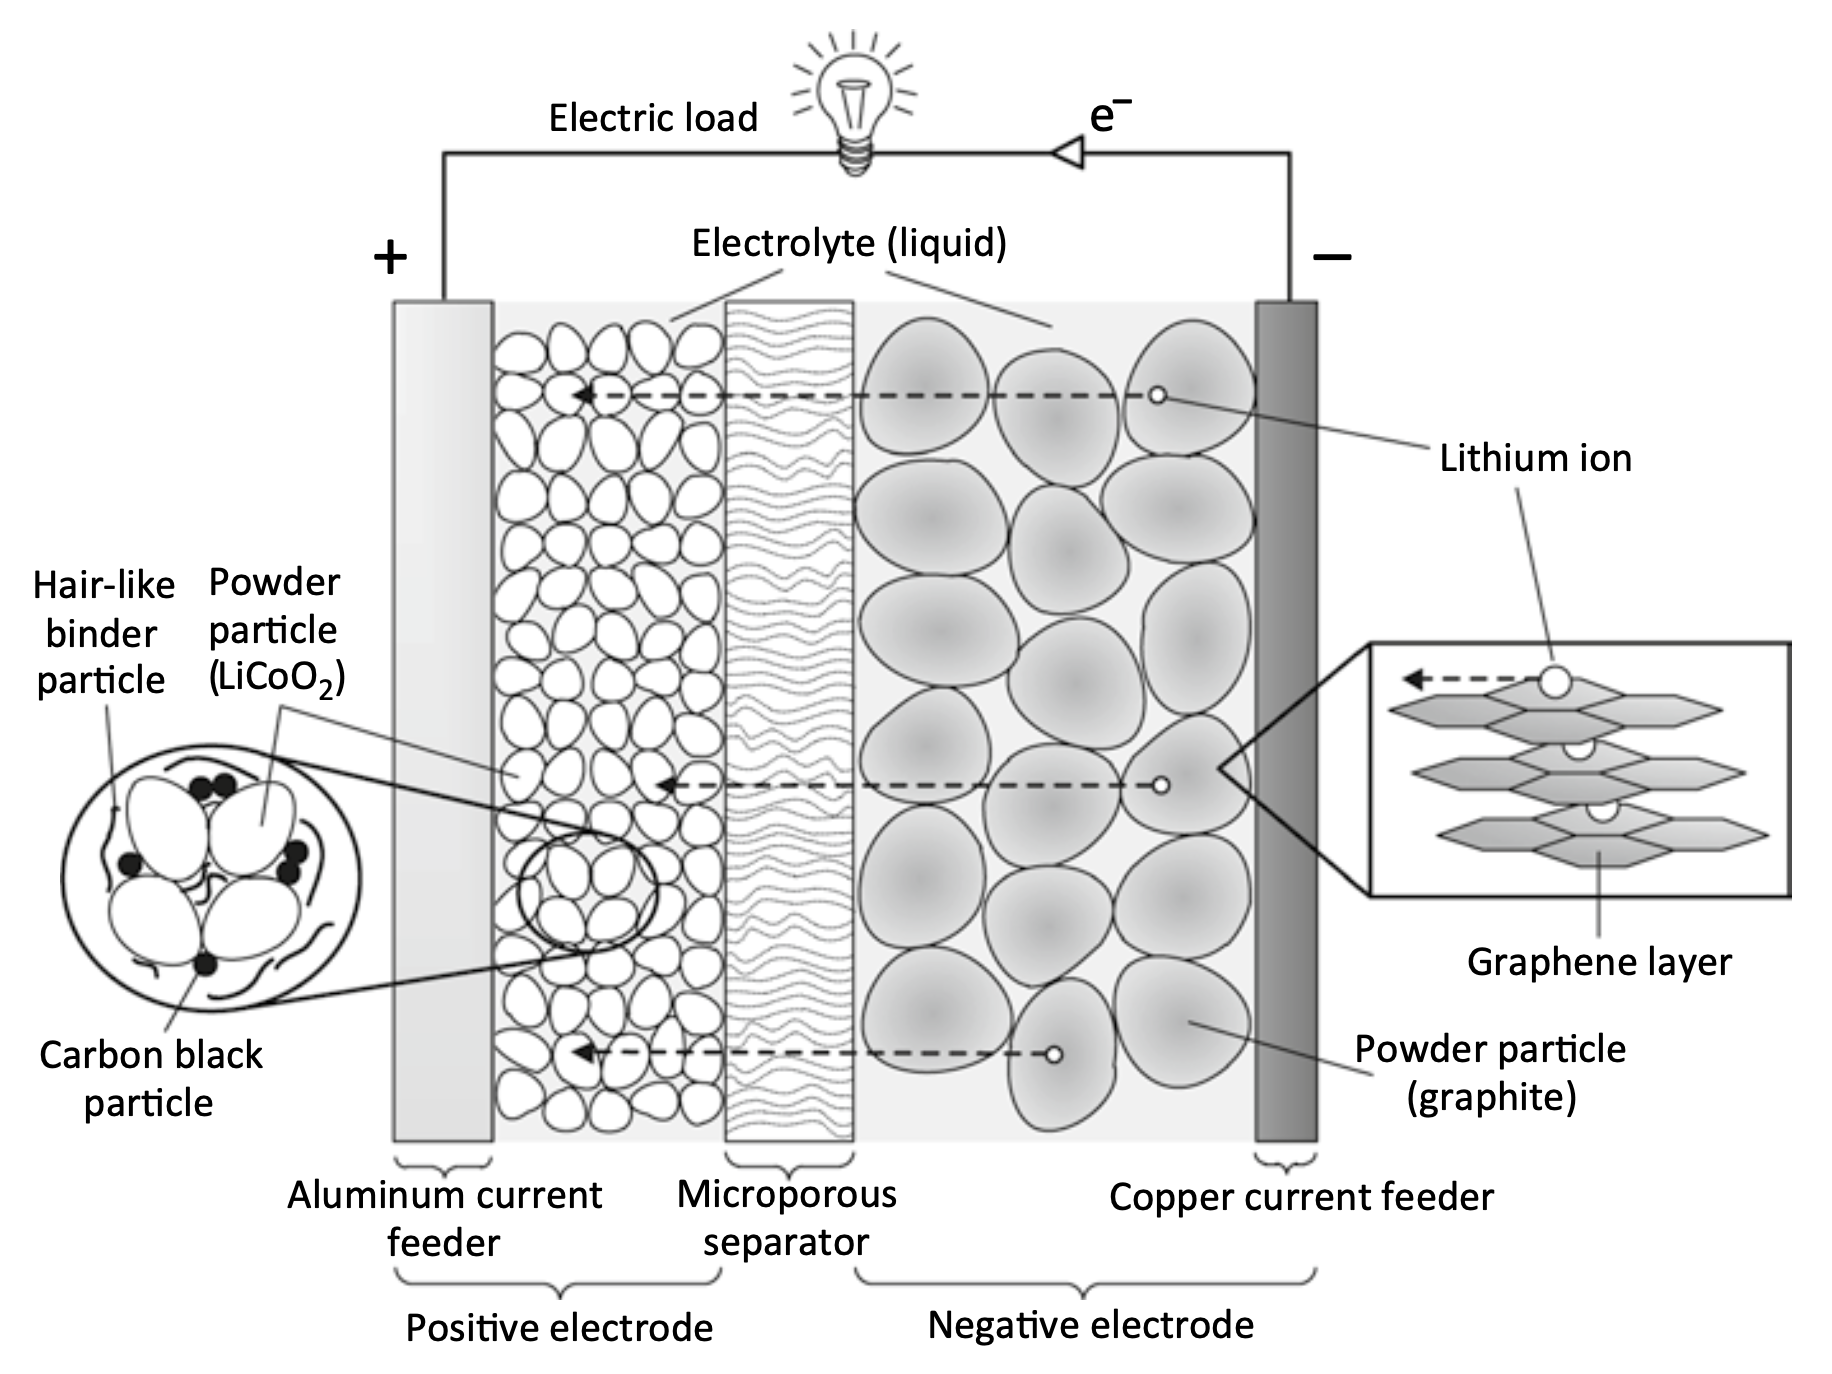
\includegraphics[width=0.8\textwidth]{Images/Chapter1/overview3.png}
    \caption{Components of a traditional lithium-ion battery during discharging. Source: Korthauer (2018) \cite{korthauer2018lithium}.}
    \label{fig:lib-overview}
\end{figure}

The electrolyte conducts the ionic component of the chemical reaction between the anode and the cathode, but it forces the electronic component to traverse an external circuit where it does work. Metallic current collectors deliver electronic current from/to the redox centers of the electrodes to/from the external circuit. These elements are used to produce cylindrical, prismatic and pouch cells. Depending on the application, a single battery cell is used or several cells are connected in series in a module. Also, a parallel connection is possible, dependent on the required capacity. Several connected modules form a battery system for auto-motive applications \cite{korthauer2018lithium,goodenough2013li}.

\subsection{Positive Electrode}
\label{sec:positive-electrode}
% See the book for articles to cite in these parts!
% This part has to be changed since it is copied from (Li-ion definitive book)
Lithium transition metal compounds are employed as positive electrode materials. These composites can develop mixed crystals over an ample composition range and can deintercalate lithium ions from the structure during the charging process. The traditional positive electrode material is lithiated cobalt oxide, LiCoO$_2$. It has a layered structure with alternating cobalt, oxygen, and lithium ion layers. During charging, lithium leaves the crystal (deintercalation); during discharging, it returns (intercalation). However, only 50\% of the lithium may be utilized. If more than half of the lithium leaves the crystal, the structure may collapse and liberate oxygen. This can cause thermal runaway, as oxygen is able to burn the electrolyte. For complete discharging, the reaction at the positive electrode is:
\begin{equation}
    \label{eq:positive-electrode}
    2\text{Li}_{0.5}\text{CoO}_2 + \text{Li}^+ + e^- \rightarrow 2\text{LiCoO}_2
\end{equation}
Thus for one mole (7 g) of active lithium, two moles (189 g) of Li$_{0.5}$CoO$_2$ are needed as host for lithium during discharge.

The use of cobalt oxide as positive electrode material is not safe. If it is kept “fully” charged as Li$_{0.5}$CoO$_2$, it reacts slowly with the electrolyte, thus losing performance. If it is slightly overcharged, there is a clear loss in capacity and service life. In case of severe overcharging, the cobalt oxide crystal collapses which can cause thermal runaway and fire. Overcharging easily happens, as there is no obvious voltage difference between normal charging and overcharging. Cobalt oxide is expensive, as cobalt ore is scarce. This problem is getting worse as the demand grows. Economics of scale do not apply here. Last but not least, cobalt is toxic.

The main commercial alternatives for cobalt oxide are listed in Table \ref{table:cathode-alternatives}. Each of the alternative materials solves some of the problems but they all are compromises. LMO is safer and very cheap but has a limited service life. NCM is safer and cheaper, but has a sloping discharge voltage. NCA is cheaper and lighter (more specific capacity, mAh/g) but it is hardly safer. LFP is very safe and slightly cheaper, but it gives 0.5 V lower voltage than cobalt oxide. At the moment, NCM and LFP seem to be the most promising candidates for large-scale batteries.

\begin{table}[H]
    \centering 
        \begin{tabular}{|c c c|}
        \hline
        \rowcolor{bluepoli!40}
        \textbf{Compound} & \textbf{Abbreviation} & \textbf{Chemical structure} \T\B \\
        \hline \hline
        Manganese oxide & LMO & LiMn$_2$O$_4$\T\B\\
        \hline
        Nickel manganese cobalt oxide & NCM & LiNi$_{1/3}$Mn$_{1/3}$Co$_{1/3}$O$_2$\T\B\\
        \hline
        Nickel cobalt aluminum oxide & NCA & LiNi$_{0.8}$Co$_{0.15}$Al$_{0.15}$O$_2$\T\B\\
        \hline
        Iron phosphate & LFP & LiFePO$_4$\T\B\\
        \hline
        \end{tabular}
        \\[10pt]
        \caption{Commercial alternatives for cobalt oxide. Source: Korthauer (2018) \cite{korthauer2018lithium}.}
        \label{table:cathode-alternatives}
    \end{table}

\subsection{Negative Electrode}
\label{sec:negative-electrode}
% See the book for articles to cite in these parts!
% This part has to be changed since it is copied from (Li-ion definitive book)
By far the most common negative electrode material is graphitic carbon. It has carbon atoms in parallel graphene layers. During charging, the lithium ions are intercalated into the graphite, between its layers. During discharging, lithium leaves the graphite. Unlike cobalt oxide, graphite is stable even without lithium, so it can be almost completely discharged. For complete discharging, the reaction at the negative electrode is:
\begin{equation}
    \label{eq:negative-electrode}
    \text{LiC}_6 \rightarrow \text{Li}^+ + e^- + 6\text{C}
\end{equation}
Thus for one mole (7 g) of active lithium, there are six moles (72 g) of carbon that act as host for the lithium during charging.

Graphite as negative electrode is not safe either. For graphite, the lithium intercalation potential is only about 80 mV more positive than the lithium metal plating potential. Even a small design failure or charging error causes deposition of metallic lithium on the electrode surface. Small amounts of metallic lithium increase the reactivity of the graphite surface, thus consuming electrolyte in secondary reactions. Large amounts of deposited lithium metal can grow as metallic peaks, “dendrites”, that short-circuit the negative and positive electrodes. This might cause excess heating and ignite the electrolyte resulting in a fire.

The potential of lithiated graphite is far beyond the stability window of the common electrolytes. During the first charging of the battery, graphite reacts with the electrolyte, building a protective layer on the graphite surface. This solid electrolyte interface (SEI) layer should prevent further secondary reactions. However, some secondary reactions take place throughout the lifetime of the battery, reducing its cyclic and calendar life.
Some commercial alternatives for graphite exist. Soft and hard carbons are used due to their slightly more positive intercalation potentials. This means less risk of lithium metal deposition and a possibility of faster charging.
However, the energy density is considerably lower when these materials are used. Lithium titanate is a very safe negative electrode material with an amazingly long service life, but the 1.4 V lower cell voltage limits the use of lithium titanate to very few applications. The newest commercial alternative, silicon, gives a formidable energy density, but low stability limits its service life.

Graphite is cheap and lightweight, especially when compared to cobalt oxide. Therefore, it can be expected that graphite retains its position as standard negative electrode material in the near future.

\subsection{Electrolyte}
\label{sec:electrolyte}
% This part has to be changed since it is copied from (Li-ion definitive book)
Electrolytes are an essential component of a lithium-ion battery. The interplay of solvent, conducting salt, and the respective additives forms a complex system. This system must be diligently chosen, and its characteristics must be combined in the most efficient way. At the same time, the electrolyte is not an independent component of the cell. It needs to be chosen in dependence on the materials for the anode and the cathode side. That, in turn, calls for close collaboration between the electrolyte manufacturer and the cell and battery developers. New challenges stem from the new materials of the next-generation batteries, e.g., high-voltage cathodes that demand suitably stable electrolytes not exhibiting a degradation tendency even at such potential levels. In addition to that, these electrolytes should ensure a passivation of the current collectors, which is a challenge on the cathode side at higher potentials. Alongside all these technological requirements, to realize future applications in electric mobility and stationary energy storage, it must be assured that the necessary numbers can actually be produced.
\cite{xu2004nonaqueous,aurbach1995study,song1999review,korthauer2018lithium}
% Here I should add the most important concepts of the underlined parts of the book

\subsection{Separator}
\label{sec:separator}


\subsection{Current Collectors}
\label{sec:current-collectors}


\subsection{Cell Geometries and Designs}
\label{sec:cell-geometries-designs}


\section{Safety and Degradation}
\label{sec:safety-degradation}

